% homework/q1rev/q1rev.tex
% Year 7 - Quarter 1 Review Packet: Mathematics Units 1-3, all of it.
%
% Goes out before the Quarter 1 Assessment (50 marks, 60 minutes, no
% calculator, Units 1-3 mixed). The assessment itself lives OUTSIDE this repo,
% in OneDrive\Desktop\Y7Tests\Maths\Q1-Assessment, because this repo is
% public. THIS PACKET SHARES NO QUESTION WITH IT: every question type on the
% assessment appears here, with different numbers and a different context, and
% nothing here is a copy of it. If you edit the assessment, check the packet
% has not become its answer sheet; if you edit the packet, check the reverse.
%
% THE LEVELS. Every question carries one of the three tags the Cambridge
% Workbook uses, so the class already knows what they mean:
%   Focus     -- the basics. A student who cannot do these starts here.
%   Practice  -- what most of the assessment looks like.
%   Challenge -- what its last page looks like, and harder.
% The teacher asked for a range skewed hard at the top, so Challenge is about
% a third of the packet by space, not a token last question. A8 and B8 are the
% hardest blocks: every puzzle on the assessment has a harder cousin there.
%
% The English is still the subject. Every language trap has a blue Word help
% box on the same page, as in every packet -- the assessment has none, so this
% is the last place the words are glossed before they are needed.
%
% Nothing here is lifted from the workbook, the Cambridge tests, or HW 1-8.
% Where a trap is reused it has new numbers.
%
% House style is shared: see homework/hw-style.tex. Method: the new-homework
% skill. Source is pure ASCII on purpose.
%
% Build:  pwsh .claude/skills/new-homework/scripts/build-hw.ps1 q1rev

\documentclass[12pt,a4paper]{article}

% -- Answer key switch -------------------------------------------------------
\newif\ifkey
\ifdefined\TEACHER\keytrue\else
  \keyfalse        % \keyfalse = student copy   |   \keytrue = teacher copy
\fi

% -- House style -------------------------------------------------------------
% homework/hw-style.tex
% Shared house style for every Year 7 homework packet. \input this from the
% packet file, right after \documentclass and the answer-key switch.
%
% Do not fork this file per packet. If a packet needs a different look, the
% question is whether every packet should have it.
%
% The choices here are deliberate and were arrived at by printing and looking:
%   * No solid dark banners. Every header is a light tint with a coloured spine
%     on the left, so colour reads clearly without flooding a school printer.
%   * No marks and no mark totals. These are practice, not exam papers.
%   * Lato at 12pt with open leading, plus mathastext so inline maths is Lato
%     too. Without mathastext every "-6 + 4" is Computer Modern serif and the
%     sheet looks half-typeset.
%   * Writing lines are spaced for Year 7 handwriting, not adult margin notes.
%   * Pages fill. \needspace is redefined below so a heading no longer drags
%     the page break up to itself, and every heading is glued to the box under
%     it. Packets built before 2026-09-30 were laid out under the old rules and
%     will reflow if rebuilt -- re-read every page if you rebuild one.
%
% Provides: \wlines \blank \tickbox \sep \qmk-free marks (none) \hwsection
% \qhead \expr, the workspace box, and the remember / wordhelp / activity /
% yourturn coloured boxes. Palette matches the lesson decks exactly.

% -- Packages ----------------------------------------------------------------
\usepackage[T1]{fontenc}
\usepackage[utf8]{inputenc}
\usepackage[default]{lato}
\usepackage[a4paper,top=1.7cm,bottom=1.7cm,left=2.0cm,right=2.0cm,headheight=15pt]{geometry}
\usepackage{amsmath,amssymb}
\usepackage{xcolor}
\usepackage[most]{tcolorbox}
\usepackage{enumitem}
\usepackage{tikz}
\usetikzlibrary{arrows.meta}
\usepackage{array}
\usepackage{tabularx}
\usepackage{fancyhdr}
\usepackage{multicol}
\usepackage{needspace}
\usepackage{graphicx}

% Make maths use Lato too. Without this, every "-6 + 4" on the page is set in
% Computer Modern serif and the sheet looks half-typeset. Must come last.
\usepackage[italic]{mathastext}

% -- \needspace, without the hole it used to leave ----------------------------
% needspace.sty writes "\vskip 0pt plus X \penalty-100" in front of every
% heading. A page that ends anywhere else is underfull with no stretch, so TeX
% scores it b=10000; a page that ends AT a heading gets that X of stretch and a
% finite badness, and wins. So any heading in roughly the bottom half of a page
% claimed the break, and the question under it moved over whole, leaving a hole
% the size of the question. \tracingpages showed it exactly (b=4531 at the
% heading, b=10000 at every later break) while building homework/q1rev, and it
% is where the half-empty pages in HW 1-8 came from.
% This keeps only the \penalty9999, which still refuses to put a heading in the
% last X of a page. Keeping a heading WITH the box under it is \nobreak's job
% now -- see \hwsection and \qhead below.
\makeatletter
\renewcommand{\needspace}[1]{\begingroup\setlength{\dimen@}{#1}%
  \vskip\dimen@\penalty9999\vskip-\dimen@\endgroup}
\makeatother

\linespread{1.06}\selectfont

% -- The Learner's Book palette (same hex values as the lesson decks) ---------
\definecolor{cbteal}{HTML}{0087A8}
\definecolor{cbpurple}{HTML}{5C2483}
\definecolor{cborange}{HTML}{C25E12}
\definecolor{cbgreen}{HTML}{4A8B23}
\definecolor{cbred}{HTML}{C8102E}
\definecolor{cbblue}{HTML}{1A5FA8}
\definecolor{rulegray}{HTML}{9AA5AD}

% -- Answer lines and blanks -------------------------------------------------
% \wlines{n} draws n ruled writing lines, spaced wide enough for Year 7
% handwriting rather than for an adult with a fine pen.
\makeatletter
\newcommand{\wlines}[1]{%
  \par\vspace{0.75em}%
  \@tempcnta=0\relax
  \@whilenum\@tempcnta<#1\do{%
    \hbox to \linewidth{\color{rulegray}\leaders\hrule height 0.5pt\hfill}%
    \vspace{1.5em}%
    \advance\@tempcnta by 1\relax}%
  \par\vspace{-0.8em}%
}
\makeatother

% \blank[width] is an inline gap to write a short answer in.
\newcommand{\blank}[1][2.6cm]{\underline{\hspace{#1}}}

% A boxed space for showing working.
\newtcolorbox{workspace}[1][3.4cm]{%
  colback=white, colframe=rulegray, boxrule=0.5pt, arc=5pt,
  height=#1, left=6pt, right=6pt, top=4pt, bottom=4pt,
  before skip=9pt, after skip=11pt}

% An empty tick box.
\newcommand{\tickbox}{\fbox{\rule{0pt}{1.15em}\rule{1.15em}{0pt}}}

% A middot separator.
\newcommand{\sep}{\,\textperiodcentered\,}

% -- Section and question headings -------------------------------------------
% Light tint plus a fat coloured spine on the left. No solid dark banner: the
% colour reads clearly but barely costs the printer anything.
% needspace keeps a heading out of the last few lines of a page. The \nobreak
% after it keeps it with whatever comes next: a remember or word-help box that
% does not fit takes its heading over with it, instead of leaving the heading
% alone at the foot of the page. (The old needspace did that by accident, and
% left a hole every time; see above.)
\newcommand{\hwsection}[2][cbteal]{%
  \needspace{8\baselineskip}%
  \par\vspace{13pt}%
  \noindent
  \begin{tcolorbox}[enhanced, nobeforeafter, width=\textwidth,
      colback=#1!7, colframe=#1!7, arc=5pt,
      borderline west={5pt}{0pt}{#1},
      left=14pt, right=10pt, top=7pt, bottom=7pt]
    {\large\bfseries\color{#1}#2}
  \end{tcolorbox}%
  \par\nobreak\vspace{9pt}}

% \qhead[colour]{A2}{Moving along the line} -- a question heading.
\newcommand{\qhead}[3][cbteal]{%
  \needspace{6\baselineskip}%
  \par\vspace{11pt}%
  \noindent{\large\bfseries\color{#1}#2}\quad{\large\bfseries #3}\par\nobreak\vspace{4pt}}

% -- Coloured boxes ----------------------------------------------------------
% Shared look: rounded, light fill, coloured rule, coloured title text on a
% pale title strip rather than a dark one.
% NOT breakable. A breakable box that cannot fit its first lines forces its own
% page break, and \nobreak cannot stop a forced break -- so the heading above
% it was left alone at the foot of the page (tested: it happens with \nobreak
% in place). Unbreakable, the page builder moves heading and box together.
% These boxes are a few lines each; none needs to split.
\tcbset{hwbox/.style={
  enhanced, arc=6pt, boxrule=1pt,
  left=11pt, right=11pt, top=8pt, bottom=8pt,
  fonttitle=\bfseries, attach boxed title to top left={xshift=12pt, yshift=-8pt},
  boxed title style={arc=4pt, boxrule=1pt, left=7pt, right=7pt, top=2pt, bottom=2pt},
  top=13pt}}

% Orange: things to remember. Matches the deck's "Write This Down".
\newtcolorbox{remember}[1][Remember from the lesson]{hwbox,
  colback=cborange!6, colframe=cborange, coltitle=cborange,
  colbacktitle=white, title={#1}}

% Blue: English help. The barrier in this class is the wording, not the maths.
\newtcolorbox{wordhelp}[1][Word help]{hwbox,
  colback=cbblue!6, colframe=cbblue, coltitle=cbblue,
  colbacktitle=white, title={#1}}

% Purple: an activity or instruction.
\newtcolorbox{activity}[1][How to do this homework]{hwbox,
  colback=cbpurple!6, colframe=cbpurple, coltitle=cbpurple,
  colbacktitle=white, title={#1}}

% Green: your turn / a friendly nudge.
\newtcolorbox{yourturn}[1][Your turn]{hwbox,
  colback=cbgreen!7, colframe=cbgreen, coltitle=cbgreen!75!black,
  colbacktitle=white, title={#1}}

% -- Shorthands --------------------------------------------------------------
\newcommand{\dC}{\,^{\circ}\mathrm{C}}          % use inside maths: $-8\dC$
\newcommand{\key}[1]{{\color{cborange}\textbf{#1}}}
\newcommand{\eng}[1]{{\color{cbblue}\textbf{#1}}}

\setlist[enumerate]{itemsep=8pt, topsep=5pt, leftmargin=*}
\setlist[itemize]{itemsep=4pt, topsep=4pt, leftmargin=*}
\renewcommand{\arraystretch}{1.45}

% -- An expression the student is asked to work from -------------------------
\newcommand{\expr}[1]{%
  \tcbox[on line, colback=cbgreen!10, colframe=cbgreen!55, boxrule=1pt, arc=4pt,
         left=9pt, right=9pt, top=4pt, bottom=4pt]{\large\bfseries $#1$}}

% -- Running head and foot ---------------------------------------------------
% The packet overrides \fancyhead[L] with its own title.
\pagestyle{fancy}
\fancyhf{}
\fancyhead[L]{\small\color{black!55}Year 7\sep Homework}
\fancyhead[R]{\small\color{black!55}Name: \blank[3.4cm]}
\fancyfoot[C]{\small\color{black!55}Page \thepage}
\renewcommand{\headrulewidth}{0pt}
\renewcommand{\headrule}{\vspace{2pt}\hbox to\headwidth{\color{cbteal!45}\leaders\hrule height 1.2pt\hfill}}


\usetikzlibrary{calc}

% -- Per-packet running head -------------------------------------------------
\fancyhead[L]{\small\color{black!55}Year 7\sep Quarter 1 Review}

% -- Fill the pages ----------------------------------------------------------
% needspace.sty writes "\vskip 0pt plus X \penalty-100" in front of every
% heading. A page that ends anywhere else is underfull with no stretch, so TeX
% scores it b=10000 -- but a page that ends AT a heading gets that X of
% stretch, a finite badness, and wins. With X = 6 lines, any heading in about
% the bottom half of a page claims the break, and the question under it moves
% over whole: a hole the size of the question. \tracingpages showed exactly
% this (b=4531 at the A8 heading against b=10000 everywhere after it), and it
% is where the half-empty pages in HW 1-8 came from.
% Here the stretch and the -100 are gone, so pages fill; the 9999 still keeps
% each heading with the X of material under it, so no heading is stranded.
% Local on purpose -- changing hw-style.tex would reflow every packet already
% printed.
\makeatletter
\renewcommand{\needspace}[1]{\begingroup\setlength{\dimen@}{#1}%
  \vskip\dimen@\penalty9999\vskip-\dimen@\endgroup}
\makeatother

% -- A group of writing lines that will not be split (see hw06.tex) ----------
\newcommand{\qlines}[1]{\par\needspace{\numexpr#1+1\relax\baselineskip}\wlines{#1}}

% -- A box to write one number or digit in -----------------------------------
\newcommand{\nbox}{\ \fbox{\rule{0pt}{1.05em}\rule{1.0em}{0pt}}\ }

% -- An answer blank on a line of its own, right-aligned (see hw08.tex) ------
\newcommand{\ansline}[1][4.4cm]{\par\vspace{2pt}\hspace*{\fill}\blank[#1]\par}

% -- A ragged-right X column (see hw08.tex) ----------------------------------
\newcolumntype{L}{>{\raggedright\arraybackslash}X}

% -- The three levels --------------------------------------------------------
% A small outlined tag at the right of a question heading. Outlined, not
% filled, for the same reason as the headings: colour without toner.
\newcommand{\levtag}[2]{%
  \tcbox[on line, colback=white, colframe=#1, boxrule=0.9pt, arc=3pt,
         left=5pt, right=5pt, top=1.5pt, bottom=1.5pt]%
        {\footnotesize\bfseries\color{#1}#2}}
\newcommand{\focus}{\levtag{cbgreen}{FOCUS}}
\newcommand{\practice}{\levtag{cbteal}{PRACTICE}}
\newcommand{\challenge}{\levtag{cbred}{CHALLENGE}}
% \evq{A1}{Title}{\focus} -- a question heading carrying its level. (Not \lq:
% that is LaTeX's left quote.) It asks for 8 lines, not \qhead's 6: most
% headings here are followed by a remember or word-help box, and a box that
% does not fit moves over whole -- leaving the heading alone at the foot of the
% page, which is what B4 did at 6. Safe because of the \needspace fix above:
% the reserve can no longer pull the page break towards itself.
\newcommand{\evq}[3]{\needspace{8\baselineskip}\qhead{#1}{#2\hfill#3}}

% -- Number lines (as hw08.tex) ----------------------------------------------
\newcommand{\numline}[2]{%
  \begin{tikzpicture}[x=0.84cm, y=0.84cm, line width=0.9pt]
    \draw[cbteal,{Latex[length=2.8mm]}-{Latex[length=2.8mm]}]
      ({#1-0.7},0) -- ({#2+0.7},0);
    \foreach \n in {#1,...,#2}{
      \draw[cbteal] (\n,-0.16) -- (\n,0.16);
      \node[below=2pt, font=\small] at (\n,-0.16) {$\n$};}
  \end{tikzpicture}}
% #1 from, #2 to, #3 the open circle, #4 where the arrow ends.
\newcommand{\numlinemark}[4]{%
  \begin{tikzpicture}[x=0.84cm, y=0.84cm, line width=0.9pt]
    \draw[cbteal,{Latex[length=2.8mm]}-{Latex[length=2.8mm]}]
      ({#1-0.7},0) -- ({#2+0.7},0);
    \foreach \n in {#1,...,#2}{
      \draw[cbteal] (\n,-0.16) -- (\n,0.16);
      \node[below=2pt, font=\small] at (\n,-0.16) {$\n$};}
    \draw[cborange, line width=1.9pt, -{Latex[length=3.2mm]}] (#3,0.46) -- (#4,0.46);
    \draw[cborange, line width=1.4pt, fill=white] (#3,0.46) circle (0.17);
  \end{tikzpicture}}

% -- A number card for the A8 puzzle -----------------------------------------
\newcommand{\card}[1]{\tcbox[on line, colback=black!5, colframe=black!60,
  boxrule=0.8pt, arc=2pt, left=8pt, right=8pt, top=4pt, bottom=4pt]{\large$#1$}}

\begin{document}

% ===========================================================================
% COVER BLOCK
% ===========================================================================
\thispagestyle{fancy}

\begin{tcolorbox}[enhanced, colback=cbpurple!7, colframe=cbpurple!7, arc=7pt,
                  borderline west={6pt}{0pt}{cbpurple},
                  left=18pt, right=14pt, top=10pt, bottom=10pt]
  {\color{cbpurple}\bfseries YEAR 7\sep UNITS 1--3\sep QUARTER 1 REVIEW}\\[5pt]
  {\color{cbpurple}\Huge\bfseries Units 1 to 3, All of It}\\[9pt]
  {\color{black!70}Mathematics 1.1--1.6 --- integers, factors, multiples, tests, roots}\\
  {\color{black!70}Mathematics 2.1--2.6 --- expressions, formulae, brackets, equations}\\
  {\color{black!70}Mathematics 3.1--3.2 --- powers of 10, place value, rounding}
\end{tcolorbox}

\vspace{4pt}
\noindent
\begin{tabularx}{\textwidth}{@{}X X@{}}
  \textbf{Name:} \blank[5.6cm] & \textbf{Class:} \blank[5.6cm] \\
  \textbf{Date given:} \blank[4.6cm] & \textbf{Date due:} \blank[5.0cm] \\
\end{tabularx}

\vspace{2pt}
\begin{activity}[How to use this packet]
  Every question has a \textbf{level}, like your Workbook. \;
  \focus\ the basics. \;
  \practice\ most of the Quarter 1 Assessment. \;
  \challenge\ its \textbf{last} questions --- do not skip them.
  \par\smallskip
  \key{No calculator} --- the assessment has none. \;
  \key{Write the calculation before the answer.} Every time.
\end{activity}

% ===========================================================================
% SECTION A -- UNIT 1
% ===========================================================================
\hwsection{Section A \textperiodcentered\ Unit 1 --- Integers, Factors, Multiples and Roots}

% -- A1 ---------------------------------------------------------------------
\evq{A1}{All four rules, all four signs}{\focus}

\begin{remember}[Two sets of rules --- do not mix them up]
  Add a negative or subtract a positive: move \key{left}. \; Subtract a negative: move
  \key{right}. \\
  \key{Two negatives make a positive} only for $\times$ and $\div$. \;
  $-6 + (-4) = -10$, not $+10$.
\end{remember}

\vspace{2pt}
\begin{multicols}{3}
\begin{enumerate}[label=(\alph*), itemsep=10pt]
  \item $-8+5 = \blank[1.5cm]$
  \item $7+(-12) = \blank[1.4cm]$
  \item $-3-(-11) = \blank[1.3cm]$
  \item $-7 \times (-8) = \blank[1.3cm]$
  \item $54 \div (-6) = \blank[1.4cm]$
  \item $-81 \div (-9) = \blank[1.2cm]$
  \item $-15+(-25) = \blank[1.1cm]$
  \item $0-(-13) = \blank[1.5cm]$
  \item $-2 \times (-3) \times (-5) = \blank[0.9cm]$
\end{enumerate}
\end{multicols}

% -- A2 ---------------------------------------------------------------------
\evq{A2}{Say it, then write it}{\practice}

\begin{wordhelp}[Word help --- these words decide the calculation]
  \begin{tabularx}{\linewidth}{@{}l@{\hspace{12pt}}X@{}}
    \eng{subtract 9 from 4} \sep \eng{6 less than $-3$} & start at the \textbf{second}
      number: $4 - 9$ and $-3 - 6$. \\
    \eng{by how many degrees} & it wants the \textbf{change}: the gap between the two
      temperatures. A gap is never negative. \\
  \end{tabularx}
\end{wordhelp}

\noindent Write the calculation, then the answer.

\vspace{4pt}
\begin{enumerate}[label=\arabic*., itemsep=10pt]
  \item Subtract 9 from 4. \hfill Calculation: \blank[4.2cm] \quad Answer: \blank[1.8cm]
  \item What is 6 less than $-3$? \hfill Calculation: \blank[4.2cm] \quad
        Answer: \blank[1.8cm]
  \item At midnight in Moscow the temperature is $-11\dC$. At noon it is $2\dC$.
        By how many degrees has the temperature risen? \\[3pt]
        Calculation: \blank[6.0cm] \quad Answer: \blank[2.2cm]
\end{enumerate}

% -- A3 ---------------------------------------------------------------------
\evq{A3}{The missing integer}{\practice}

\noindent Write the missing integer in each box. Check it by putting it back in.

\vspace{6pt}
\begin{multicols}{3}
\begin{enumerate}[label=(\alph*), itemsep=13pt]
  \item \nbox $\times\ (-4) = 36$
  \item $-48 \div{}$ \nbox $= -6$
  \item \nbox $\div\ (-5) = 7$
  \item $6 \times{}$ \nbox $= -42$
  \item \nbox $-\ 8 = -3$
  \item $-10 +{}$ \nbox $= -25$
\end{enumerate}
\end{multicols}

% -- A4 ---------------------------------------------------------------------
\evq{A4}{The LCM and the HCF, from the lists}{\focus}

\begin{remember}[One list stops, the other never does]
  \key{Multiples} never stop: we want the \key{lowest} common one, the \key{LCM}. \;
  \key{Factors} stop: we want the \key{highest}, the \key{HCF}.
\end{remember}

\vspace{2pt}
\noindent\textbf{(a)} Multiples of 8: \blank[6.4cm] \;\; Multiples of 14: \blank[3.4cm]

\vspace{5pt}
\noindent\hspace*{1.2em}The LCM of 8 and 14 is \blank[2.2cm]

\vspace{9pt}
\noindent\textbf{(b)} Factors of 36: \blank[6.2cm] \;\; Factors of 54: \blank[3.6cm]

\vspace{5pt}
\noindent\hspace*{1.2em}The HCF of 36 and 54 is \blank[2.2cm]

\vspace{9pt}
\noindent\textbf{(c)} Find the LCM of 9 and 15. \hfill \blank[2.4cm] \quad
\textbf{(d)} Find the HCF of 28 and 42. \hfill \blank[2.4cm]

\vspace{9pt}
\noindent\textbf{(e)} Draw a ring around \textbf{each} number that is a common factor of 48
and 72.

\vspace{7pt}
\noindent\hspace*{2.4em}\large 3\hspace{1.4cm}8\hspace{1.4cm}9\hspace{1.4cm}16\hspace{1.4cm}24\hspace{1.4cm}36\normalsize

% -- A5 ---------------------------------------------------------------------
\evq{A5}{Which one does the question want?}{\practice}

\begin{wordhelp}[Word help --- the words that tell you which one]
  \eng{together again} \sep \eng{at the same time} \sep \eng{the same number of each}
  --- something \textbf{repeating}. You want the \key{LCM}. \\
  \eng{equal groups} \sep \eng{as large as possible} \sep \eng{none left over}
  \sep \eng{none wasted} --- something being \textbf{split up}. You want the \key{HCF}.
\end{wordhelp}

\noindent Tick \textbf{HCF} or \textbf{LCM}, then work out the answer.

\vspace{6pt}
\noindent
\begin{tabularx}{\textwidth}{|L|>{\centering\arraybackslash}p{1.05cm}|>{\centering\arraybackslash}p{1.05cm}|>{\centering\arraybackslash}p{2.3cm}|}
  \hline
  \textbf{The question} & \textbf{HCF} & \textbf{LCM} & \textbf{Answer} \\
  \hline
  One light flashes every 4 seconds and another every 10 seconds. They flash together
  now. After how many seconds will they next flash together? & & & \\
  \hline
  Mr Bowen has 30 bananas and 45 mangoes. He makes identical fruit bags, using all
  the fruit. What is the greatest number of bags he can make? & & & \\
  \hline
  Sausages come in packs of 6 and bread rolls in packs of 8. Mr Bowen wants the same
  number of each. What is the smallest number of sausages he can buy? & & & \\
  \hline
\end{tabularx}

% -- A6 ---------------------------------------------------------------------
\evq{A6}{Tests for divisibility}{\practice}

\noindent\textbf{(a)} Tick ($\checkmark$) where the number divides exactly. Use the
tests --- do \textbf{not} do the divisions.

\vspace{6pt}
\noindent
\begin{tabularx}{\textwidth}{|p{2.4cm}|X|X|X|X|X|X|X|}
  \hline
  \textbf{Number} & \textbf{2} & \textbf{3} & \textbf{4} & \textbf{5} & \textbf{6} &
  \textbf{9} & \textbf{10} \\
  \hline
  $4356$ \rule[-0.7em]{0pt}{2.1em} & & & & & & & \\ \hline
  $7290$ \rule[-0.7em]{0pt}{2.1em} & & & & & & & \\ \hline
  $3015$ \rule[-0.7em]{0pt}{2.1em} & & & & & & & \\ \hline
\end{tabularx}

\vspace{10pt}
\noindent\textbf{(b)} The number \; 4\nbox 8 \; is divisible by 3. Find \textbf{all}
the possible missing digits.
\ansline[4.0cm]

\vspace{6pt}
\noindent\textbf{(c)} Show that $62\,417$ is \textbf{not} divisible by 3. Do not divide.
\qlines{1}

% -- A7 ---------------------------------------------------------------------
\evq{A7}{Squares, cubes and roots}{\focus}

\begin{remember}[Rooting is squaring run backwards]
  $9^2 = 81$, so $\sqrt{81} = 9$. \quad $4^3 = 64$, so $\sqrt[3]{64} = 4$. \quad
  $3^3$ is $3 \times 3 \times 3 = 27$, \key{not} $3 \times 3$.
\end{remember}

\vspace{2pt}
\begin{multicols}{3}
\begin{enumerate}[label=(\alph*), itemsep=10pt]
  \item $13^2 = \blank[1.5cm]$
  \item $5^3 = \blank[1.5cm]$
  \item $\sqrt{121} = \blank[1.4cm]$
  \item $\sqrt[3]{1000} = \blank[1.3cm]$
  \item $3^3 - 4^2 = \blank[1.2cm]$
  \item $\sqrt{36} + \sqrt[3]{8} = \blank[1.0cm]$
\end{enumerate}
\end{multicols}

\vspace{2pt}
\noindent\textbf{(g)} Explain why 25 is a square number but \textbf{not} a cube number.
\qlines{2}

% -- A8 ---------------------------------------------------------------------
% The Unit 1 puzzles. Each is a harder cousin of a question on the assessment:
% the HCF/LCM pair, the product-and-sum pair (twice -- once with both numbers
% negative), the missing digit (here with 15, which has no test of its own and
% needs 3 AND 5), the root-to-root question (here with 729, where the second
% root has to be found, not remembered), and the card puzzle from the Stage 7
% end-of-year paper.
\evq{A8}{Unit 1 puzzles}{\challenge}

\begin{wordhelp}[Word help]
  \eng{product} --- the answer to a \textbf{multiplication}. \quad
  \eng{sum} --- the answer to an \textbf{addition}.
\end{wordhelp}

% Every puzzle is one minipage, so its question and its box cannot land on
% different pages. The short ones sit in pairs, side by side: none of them
% needs a full width to work in, and the packet has a 10-page target.
\noindent
\begin{minipage}{\textwidth}
  \textbf{1.} The HCF of two numbers is 5. The LCM of the two numbers is 60. Both
  numbers are bigger than 5 and smaller than 60. Find the two numbers.
  \begin{workspace}[1.8cm]\end{workspace}
\end{minipage}

\vspace{7pt}
\noindent
\begin{minipage}[t]{0.485\textwidth}
  \textbf{2.} The product of two integers is $-42$. Their sum is $1$. Find the two
  integers.
  \begin{workspace}[1.8cm]\end{workspace}
\end{minipage}\hfill
\begin{minipage}[t]{0.485\textwidth}
  \textbf{3.} The product of two integers is $24$. Their sum is $-10$. Find the two
  integers.
  \begin{workspace}[1.8cm]\end{workspace}
\end{minipage}

\vspace{7pt}
\noindent
\begin{minipage}[t]{0.485\textwidth}
  \textbf{4.} The number \; 2\nbox 5 \; is divisible by 15. Find \textbf{all} the
  possible missing digits. \\ \emph{Hint:} $15 = 3 \times 5$.
  \begin{workspace}[1.8cm]\end{workspace}
\end{minipage}\hfill
\begin{minipage}[t]{0.485\textwidth}
  \textbf{5.} The cube root of a number is 9. Work out the \textbf{square} root of
  the number.
  \begin{workspace}[1.8cm]\end{workspace}
\end{minipage}

\vspace{7pt}
% The card puzzle is one block: split across a page, the cards land on one
% side of the sheet and the statements on the other.
\noindent
\begin{minipage}{\textwidth}
  \textbf{6.} Here are eight number cards. Use each card \textbf{once} to make all
  four statements true.
  \par\vspace{6pt}
  \noindent\hspace*{0.2em}\card{27}\ \card{-5}\ \card{3}\ \card{-2}\
  \card{8}\ \card{4}\ \card{-9}\ \card{6}
  \par\vspace{8pt}
  \begin{tabular}{@{}l@{\hspace{2.2cm}}l@{}}
    (a) \nbox $+$ \nbox $= -11$ \rule[-0.6em]{0pt}{2.2em} &
    (b) \nbox $\times$ \nbox $= -40$ \\
    (c) \nbox$^{\,3}$ $+$ \nbox $= 70$ \rule[-0.6em]{0pt}{2.6em} &
    (d) $\sqrt[3]{\phantom{0}}$\nbox $\times$ \nbox $= 9$ \\
  \end{tabular}
\end{minipage}

% ===========================================================================
% SECTION B -- UNIT 2
% ===========================================================================
\hwsection{Section B \textperiodcentered\ Unit 2 --- Expressions, Formulae and Equations}

% -- B1 ---------------------------------------------------------------------
\evq{B1}{Expression, equation or formula?}{\focus}

\begin{remember}[Three words, three different things]
  \key{Expression}: \textbf{no} $=$ sign. \; \key{Equation}: $=$ and one letter to
  \textbf{find}. \; \key{Formula}: $=$ and a \textbf{rule} joining letters.
\end{remember}

% The instruction is the table's own first header cell, so it cannot be left
% behind at the foot of a page while the table goes over.
\vspace{2pt}
\noindent
\begin{tabularx}{\textwidth}{|L|>{\centering\arraybackslash}p{2.6cm}|>{\centering\arraybackslash}p{2.6cm}|>{\centering\arraybackslash}p{2.6cm}|}
  \hline
  \textbf{Tick one box in each row.} & \textbf{Expression} & \textbf{Equation} & \textbf{Formula} \\
  \hline
  $3y + 4$ \rule[-0.6em]{0pt}{1.9em}        & & & \\ \hline
  $3y + 4 = 19$ \rule[-0.6em]{0pt}{1.9em}   & & & \\ \hline
  $A = lw$ \rule[-0.6em]{0pt}{1.9em}        & & & \\ \hline
  $P = 2l + 2w$ \rule[-0.6em]{0pt}{1.9em}   & & & \\ \hline
  $12 = 2k$ \rule[-0.6em]{0pt}{1.9em}       & & & \\ \hline
\end{tabularx}

% -- B2 ---------------------------------------------------------------------
\evq{B2}{Mr Bowen thinks of a number}{\practice}

\begin{wordhelp}[Word help --- which number comes first?]
  \begin{tabularx}{\linewidth}{@{}l@{\hspace{12pt}}X@{}}
    \eng{subtract 5 from it} \sep \eng{subtract it from 5} & \; $n - 5$ \sep $5 - n$ \\
    \eng{subtract the result from 40}  & start with 40: \; $40 - $ \textbf{everything so far} \\
  \end{tabularx}
\end{wordhelp}

\noindent Mr Bowen thinks of a number, $n$. Write an expression for the number he gets
when he:

\vspace{4pt}
\begin{multicols}{2}
\begin{enumerate}[label=(\alph*), itemsep=12pt]
  \item subtracts 5 from it \hfill \blank[2.6cm]
  \item subtracts it from 5 \hfill \blank[2.6cm]
\end{enumerate}
\end{multicols}

\vspace{-4pt}
\begin{enumerate}[label=(\alph*), start=3, itemsep=10pt]
  \item multiplies it by 3, then subtracts 2 \hfill \blank[3.6cm]
  \item divides it by 5, then adds 9 \hfill \blank[3.6cm]
  \item multiplies it by 2, then subtracts the result from 40 \hfill \blank[3.6cm]
  \item adds 4, then multiplies the result by 3 \hfill \blank[3.6cm]
\end{enumerate}

% -- B3 ---------------------------------------------------------------------
\evq{B3}{Put the number in}{\practice}

\begin{remember}[A negative goes in with its brackets]
  If $b = -3$: \; $4b = 4 \times (-3) = -12$ \; and \; $10 - b = 10 - (-3) = 13$.
  \; $3a$ with $a = 5$ is $15$, \key{never} $35$.
\end{remember}

\vspace{2pt}
\noindent Work out the value of each expression when \; $a = 5$, \; $b = -3$ \; and
\; $c = 4$.

\vspace{6pt}
\begin{multicols}{3}
\begin{enumerate}[label=(\alph*), itemsep=13pt]
  \item $3a - c$ \hfill \blank[1.5cm]
  \item $4b$ \hfill \blank[1.5cm]
  \item $c - b$ \hfill \blank[1.5cm]
  \item $2a - 3b$ \hfill \blank[1.5cm]
  \item $ab + c$ \hfill \blank[1.5cm]
  \item $\dfrac{20}{c} - b$ \hfill \blank[1.5cm]
\end{enumerate}
\end{multicols}

% -- B4 ---------------------------------------------------------------------
\evq{B4}{Which way round is the formula?}{\practice}

\begin{wordhelp}[Word help --- read it as a sentence]
  A formula says \textbf{how to get the thing on the left}. Test each one with a
  number you know: 2 kg is 2000 g.
\end{wordhelp}

\noindent\textbf{(a)} Which formula is correct, \textbf{A} or \textbf{B}? \hfill
\blank[2.2cm]

\vspace{4pt}
\noindent\hspace*{1.2em}\begin{tabular}{@{}ll@{}}
  \textbf{A} & number of kilograms $= 1000 \times{}$ number of grams \\
  \textbf{B} & number of grams $= 1000 \times{}$ number of kilograms \\
\end{tabular}

\vspace{8pt}
\noindent\textbf{(b)} Write the correct formula using letters. Use $g$ for grams and
$k$ for kilograms.
\ansline[4.0cm]

\vspace{9pt}
\noindent\textbf{(c)} Use your formula to find the number of grams in $4.5$ kg.
\hfill \blank[3.2cm]


% -- B5 ---------------------------------------------------------------------
\evq{B5}{Collect like terms}{\focus}

\begin{remember}[Every sign travels with its own term]
  $7x + 5y - 3x + y = \key{4x + 6y}$: \; $+7x$ and $-3x$, then $+5y$ and $+y$. \;
  $y$ means $1y$.
\end{remember}

\vspace{2pt}
\begin{multicols}{2}
\begin{enumerate}[label=(\alph*), itemsep=12pt]
  \item $9y - y$ \hfill \blank[2.8cm]
  \item $4a + 2b + a$ \hfill \blank[2.8cm]
  \item $6p - 2q - 4p + 5q$ \hfill \blank[2.4cm]
  \item $3xy + 5yx - 2xy$ \hfill \blank[2.4cm]
  \item $7m + 3 - 2m - 8$ \hfill \blank[2.4cm]
  \item $4a^2 + 3a - a^2 + 2a$ \hfill \blank[2.2cm]
\end{enumerate}
\end{multicols}

\vspace{2pt}
\noindent\textbf{(g)} Mr Bowen simplifies \; $5k - 2j + 3k + j$ \; and gets
\; $8k - 3j$. \; What is the correct answer, and what did he do wrong?
\qlines{2}

% -- B6 ---------------------------------------------------------------------
\evq{B6}{Expand, then collect}{\practice}

\begin{remember}[The number outside multiplies \textbf{everything} inside]
  $3(x - 2) = 3x - 6$. \; Expand first, then collect: \;
  $3(x + 2) + 4x = 3x + 6 + 4x = 7x + 6$.
\end{remember}

\vspace{2pt}
\begin{multicols}{2}
\begin{enumerate}[label=(\alph*), itemsep=12pt]
  \item $7(y - 3)$ \hfill \blank[3.0cm]
  \item $5(3 - 2m)$ \hfill \blank[3.0cm]
\end{enumerate}
\end{multicols}

\vspace{-4pt}
\noindent Expand and simplify.
\begin{enumerate}[label=(\alph*), start=3, itemsep=6pt]
  \item $2(4p + 1) + 3p$ \hfill \blank[4.0cm]
  \item $6(x - 2) - 2x$ \hfill \blank[4.0cm]
  \item $3(2x + 1) + 2(x + 4)$ \hfill \blank[4.0cm]
  \item Mr Bowen expands \; $5(2k - 3)$ \; and gets \; $10k - 3$. \; Is he correct?
        Explain.
        \qlines{2}
\end{enumerate}

% -- B7 ---------------------------------------------------------------------
\evq{B7}{Solve it}{\focus}

\begin{remember}[Last on, first off --- then check]
  $2a + 4 = 18$: undo the \key{add 4} first. \; $18 - 4 = 14$, \;
  $14 \div 2 = \mathbf{7}$. \; Check: $2 \times 7 + 4 = 18$ \;$\checkmark$
\end{remember}

\vspace{2pt}
\begin{multicols}{2}
\begin{enumerate}[label=(\alph*), itemsep=11pt]
  \item $y - 7 = 19$ \hfill $y = \blank[1.8cm]$
  \item $\dfrac{k}{4} = 8$ \hfill $k = \blank[1.8cm]$
  \item $3a + 7 = 34$ \hfill $a = \blank[1.8cm]$
  \item $5b - 8 = 42$ \hfill $b = \blank[1.8cm]$
  \item $2c + 15 = 51$ \hfill $c = \blank[1.8cm]$
  \item $7d - 4 = 52$ \hfill $d = \blank[1.8cm]$
\end{enumerate}
\end{multicols}

\vspace{2pt}
\noindent\textbf{(g)} This one is written the other way round. \quad $40 = 6n - 2$
\hfill $n = \blank[1.8cm]$

% -- B8 ---------------------------------------------------------------------
% Every part is two jobs: write the equation, then solve it. (a) is the
% isosceles triangle from the Cambridge papers; (b) is the age question with
% pets, and it asks for the dog, so the letter is not the answer; (c) needs a
% bracket expanded before it can be solved, and is the hardest in Section B. A "Mr Bowen thinks of a number,
% multiplies by 4, adds 13, gets 49" part came out for the page target: B2
% writes those expressions and B7 solves those equations.
\evq{B8}{Write the equation, then solve it}{\challenge}

\begin{wordhelp}[Word help]
  \eng{isosceles} --- a triangle with \textbf{two} equal sides. \quad
  \eng{equilateral} --- \textbf{all three} sides equal. \\
  \eng{perimeter} --- the distance \textbf{all the way round}. \quad
  \eng{4 years older than} --- add 4.
\end{wordhelp}

\noindent
\begin{minipage}[t]{0.40\textwidth}
  \vspace{0pt}
  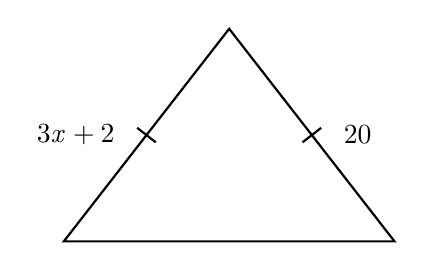
\begin{tikzpicture}
    \coordinate (A) at (0,0);
    \coordinate (B) at (4.2,0);
    \coordinate (C) at (2.1,2.7);
    \draw[thick] (A) -- (B) -- (C) -- cycle;
    \coordinate (M1) at ($(A)!0.5!(C)$);
    \coordinate (M2) at ($(B)!0.5!(C)$);
    \draw[thick] ($(M1)!0.15cm!90:(C)$) -- ($(M1)!0.15cm!-90:(C)$);
    \draw[thick] ($(M2)!0.15cm!90:(C)$) -- ($(M2)!0.15cm!-90:(C)$);
    \node[left=8pt] at (M1) {$3x + 2$};
    \node[right=8pt] at (M2) {$20$};
  \end{tikzpicture}
\end{minipage}%
\begin{minipage}[t]{0.58\textwidth}
  \vspace{0pt}
  \textbf{(a)} This triangle is isosceles. The marked sides are equal.
  \par\vspace{4pt}
  Write an equation in $x$: \blank[3.6cm]
  \par\vspace{8pt}
  Solve it: \hfill $x = \blank[2.2cm]$
\end{minipage}

\vspace{12pt}
\noindent
\begin{minipage}{\textwidth}
  \textbf{(b)} Mr Bowen's cat is $c$ years old. His dog is 4 years older than the
  cat. \\
  \hspace*{1.2em}(i) Write an expression for the dog's age. \hfill \blank[3.0cm] \\[6pt]
  \hspace*{1.2em}(ii) The sum of their ages is 18. How old is the \textbf{dog}?
  \begin{workspace}[1.6cm]\end{workspace}
\end{minipage}

\vspace{7pt}
\noindent
\begin{minipage}{\textwidth}
  \textbf{(c)} An equilateral triangle has sides of length $2y + 1$ cm. Its
  perimeter is 45 cm. Write an equation, then find $y$.
  \begin{workspace}[1.8cm]\end{workspace}
\end{minipage}

% -- B9 ---------------------------------------------------------------------
\evq{B9}{Inequalities}{\practice}

\begin{wordhelp}[Word help]
  $<$ \eng{is less than} \quad $>$ \eng{is greater than} \quad
  \eng{integer} --- a whole number: negative, zero or positive. \\
  An \textbf{open circle} means that number is \textbf{not} included.
\end{wordhelp}

\noindent
\begin{minipage}[c]{0.62\textwidth}\numlinemark{-6}{2}{-3}{-6.6}\end{minipage}%
\begin{minipage}[c]{0.36\textwidth}\textbf{(a)} Write the inequality this number
  line shows. Use $x$. \\[4pt] \blank[3.4cm]\end{minipage}

\vspace{9pt}
\noindent
\begin{minipage}[c]{0.62\textwidth}\numline{-5}{3}\end{minipage}%
\begin{minipage}[c]{0.36\textwidth}\textbf{(b)} Show \; $x > -2$ \; on this
  number line.\end{minipage}

\vspace{10pt}
\noindent\textbf{(c)} Write the integer asked for.

\vspace{2pt}
\begin{multicols}{2}
\begin{enumerate}[label=(\roman*), itemsep=10pt]
  \item $n > 3.7$. Smallest? \hfill \blank[1.8cm]
  \item $y < -6$. Largest? \hfill \blank[1.8cm]
  \item $t > -2.5$. Smallest? \hfill \blank[1.8cm]
  \item $p < 0$. Largest? \hfill \blank[1.8cm]
\end{enumerate}
\end{multicols}

\noindent\textbf{(d)} \challenge\; $x$ is an integer. \; $x > -3$ \; and \; $x < 2$.
\; Write \textbf{all} the values $x$ could be.
\ansline[6.0cm]

% ===========================================================================
% SECTION C -- UNIT 3
% ===========================================================================
\hwsection{Section C \textperiodcentered\ Unit 3 --- Place Value and Rounding}

% -- C1 ---------------------------------------------------------------------
\evq{C1}{Powers of 10: move the digits}{\focus}

\begin{remember}[The point never moves --- the digits do]
  $5.3 \times 10^2 = 530$, {\color{cbred}\bfseries not 5.300.} \; $\times$ moves the
  digits \key{left}, $\div$ moves them \key{right}; the power says \key{how far}.
\end{remember}

\vspace{2pt}
\noindent\textbf{(a)} $10^6$ as an ordinary number: \blank[3.0cm] \hfill
\textbf{(b)} $10\,000$ as a power of 10: \blank[1.8cm]

\vspace{6pt}
\begin{multicols}{3}
\begin{enumerate}[label=(\alph*), start=3, itemsep=12pt]
  \item $0.73 \times 100 = \blank[1.2cm]$
  \item $2.08 \times 10^3 = \blank[1.2cm]$
  \item $59 \times 10^2 = \blank[1.4cm]$
  \item $7.4 \div 10 = \blank[1.6cm]$
  \item $62 \div 10^3 = \blank[1.4cm]$
  \item $3 \div 10^2 = \blank[1.6cm]$
\end{enumerate}
\end{multicols}

% -- C2 ---------------------------------------------------------------------
\evq{C2}{The mass ladder}{\practice}

\begin{remember}[Each step on the ladder is $\times 1000$ or $\div 1000$]
  t \;$\xrightarrow{\;\times 1000\;}$\; kg \;$\xrightarrow{\;\times 1000\;}$\; g
  \;$\xrightarrow{\;\times 1000\;}$\; mg \qquad To a \textbf{smaller} unit, the number
  gets \textbf{bigger}.
\end{remember}

\vspace{2pt}
\begin{multicols}{2}
\begin{enumerate}[label=(\alph*), itemsep=12pt]
  \item $4.2$ kg $= \blank[2.2cm]$ g
  \item $750$ g $= \blank[2.2cm]$ kg
  \item $3$ t $= \blank[2.2cm]$ kg
  \item $2500$ mg $= \blank[2.2cm]$ g
\end{enumerate}
\end{multicols}

\noindent\textbf{(e)} \challenge\; Two steps: \; $0.06$ kg $= \blank[2.8cm]$ mg

% -- C3 ---------------------------------------------------------------------
\evq{C3}{Round it}{\practice}

\begin{remember}[Look at the next digit --- and keep the zeros]
  $34.9892$ to \key{1 decimal place} is \key{35.0}, not 35. The $.0$ shows you
  rounded to one place.
\end{remember}

\vspace{2pt}
\noindent
\begin{tabularx}{\textwidth}{|>{\raggedright\arraybackslash}p{3.6cm}|X|X|X|}
  \hline
  \textbf{To 1 decimal place} \rule[-0.7em]{0pt}{2.1em} & $6.48$ & $13.95$ & $0.349$ \\ \hline
  \rule[-0.7em]{0pt}{2.0em} & & & \\ \hline
  \textbf{To 2 decimal places} \rule[-0.7em]{0pt}{2.1em} & $4.736$ & $18.0952$ & $2.998$ \\ \hline
  \rule[-0.7em]{0pt}{2.0em} & & & \\ \hline
\end{tabularx}

% -- C4 ---------------------------------------------------------------------
\evq{C4}{One place further}{\practice}

\begin{wordhelp}[Word help --- \emph{correct to 2 decimal places}]
  \textbf{exactly two} digits after the point. To decide the second, you need the
  \textbf{third}: divide to three places, then round.
\end{wordhelp}

\vspace{2pt}
\noindent
\begin{minipage}[t]{0.32\textwidth}
  (a) $38 \div 7$, to 2 d.p.
  \begin{workspace}[2.1cm]\end{workspace}
\end{minipage}\hfill
\begin{minipage}[t]{0.32\textwidth}
  (b) $25 \div 6$, to 2 d.p.
  \begin{workspace}[2.1cm]\end{workspace}
\end{minipage}\hfill
\begin{minipage}[t]{0.32\textwidth}
  (c) $50 \div 3$, to 1 d.p.
  \begin{workspace}[2.1cm]\end{workspace}
\end{minipage}

% -- C5 ---------------------------------------------------------------------
\evq{C5}{Mr Bowen's homework}{\practice}

\noindent \textbf{One} of these four is right. Find it, and correct the other three.

\vspace{4pt}
\begin{multicols}{2}
\begin{enumerate}[label=(\alph*), itemsep=11pt]
  \item $4.9 \times 1000 = 4.9000$ \hfill \blank[2.0cm]
  \item $72 \div 100 = 7.2$ \hfill \blank[2.0cm]
  \item $3.97$ to 1 d.p. $= 3.10$ \hfill \blank[2.0cm]
  \item $0.0854$ to 2 d.p. $= 0.09$ \hfill \blank[2.0cm]
\end{enumerate}
\end{multicols}

% One block: the sentence to finish must not land on a page without its
% prompt.
\vspace{2pt}
\noindent
\begin{minipage}{\textwidth}
  \textbf{(e)} The mistake Mr Bowen made in (a) is \blank[8.6cm]
  \par\vspace{11pt}
  \hspace*{1.2em}\blank[15.4cm]
\end{minipage}

% -- C6 ---------------------------------------------------------------------
\evq{C6}{In between}{\challenge}

\begin{enumerate}[label=(\alph*), itemsep=11pt]
  \item $2.38 < x < 2.39$. \; Write a possible value for $x$. \hfill \blank[3.0cm]
  \item Write \textbf{three} different numbers between $0.1$ and $0.11$.
        \hfill \blank[6.0cm]
  \item Mr Bowen rounds a number to 1 decimal place and gets $5.4$. What is the
        \textbf{smallest} number it could have been? \hfill \blank[3.0cm]
\end{enumerate}

% ===========================================================================
% SECTION D -- MIXED
% ===========================================================================
\hwsection[cbgreen]{Section D \textperiodcentered\ All Three Units at Once}

% -- D1 ---------------------------------------------------------------------
\evq{D1}{Word problems}{\challenge}

\begin{enumerate}[label=\textbf{\arabic*.}, itemsep=8pt]
  \item \textbf{Harbin.} At 5 am the temperature is $-18\dC$. By 2 pm it has risen by
        11 degrees. By 11 pm it has fallen by 6 degrees. \\
        \textbf{(a)} What is the temperature at 11 pm? \quad
        \textbf{(b)} What is the difference between the warmest and the coldest of
        these three temperatures?
        \begin{workspace}[1.6cm]\end{workspace}
  % The deadpan one. Everything it needs was taught: an equation with like terms
  % in it, and then reading to the end of the question.
  \item \textbf{The mangoes.} Mr Bowen has $x$ mangoes. His neighbour has three times as
        many mangoes as Mr Bowen. Together they have 48 mangoes. \\
        \textbf{(a)} Write an equation. \quad
        \textbf{(b)} How many mangoes does the neighbour have? \\
        \textbf{(c)} Mr Bowen then eats all of his own mangoes in one afternoon. How
        many mangoes does Mr Bowen have now?
        \begin{workspace}[1.7cm]\end{workspace}
\end{enumerate}

% -- D2 ---------------------------------------------------------------------
\evq{D2}{Now you write the question}{\challenge}

\noindent Write a word problem for \; \expr{3n - 4 = 20}

\begin{yourturn}[The rules]
  A \textbf{real} situation \sep full sentences \sep ends in a \textbf{question} \sep
  comes out at $n = 8$
\end{yourturn}
\qlines{3}

% A half-page "Before the Assessment -- What Can You Do?" tick-list (one row per
% lesson, 1.1 to 3.2, pointing at the questions for each) stood here. It came
% out for the 10-page target: every question heading already names its unit,
% so it was a map of the packet rather than more practice.

% ===========================================================================
% ANSWER KEY (teacher copy only)
% ===========================================================================
\ifkey
\newpage
\hwsection[cbred]{Answer Key --- Teacher Copy}

\linespread{1.0}\selectfont
\setlist[enumerate]{itemsep=2pt, topsep=3pt, leftmargin=*}
\setlist[itemize]{itemsep=2pt, topsep=3pt, leftmargin=*}

\noindent{\small The Quarter 1 Assessment shares no question with this packet, but
every type on it is here. A student who can do the PRACTICE questions can pass it;
the CHALLENGE questions are harder than anything on it, on purpose.}

\qhead[cbred]{A1}{All four rules, all four signs}
\noindent (a) $-3$ \quad (b) $-5$ \quad (c) $8$ \quad (d) $56$ \quad (e) $-9$ \quad
(f) $9$ \quad (g) $-40$ \quad (h) $13$ \quad (i) $-30$

\smallskip
\noindent{\small (g) is the one to watch: $-15+(-25)$ is an \emph{addition}, so a
student who writes $40$ has used the multiplying rule on it. (i) has three negatives
and comes out negative.}

\qhead[cbred]{A2}{Say it, then write it}
\noindent 1. $4 - 9 = -5$ \quad 2. $-3 - 6 = -9$ \quad
3. $2 - (-11) = 13$ degrees

\smallskip
\noindent{\small 1 and 2 are the reversed-order trap: $9 - 4$ or $6 - (-3)$ is an
\textbf{English} error, so make the student re-read the sentence rather than
correcting the sum. In 3, $-9$ means the two temperatures were added; the question
asks for the change.}

\qhead[cbred]{A3}{The missing integer}
\noindent (a) $-9$ \quad (b) $8$ \quad (c) $-35$ \quad (d) $-7$ \quad (e) $5$ \quad
(f) $-15$

\smallskip
\noindent{\small (b) and (c) are where the size comes easily and the sign does not.
(e) and (f) are adding and subtracting, not the times rules.}

\qhead[cbred]{A4}{The LCM and the HCF}
\noindent (a) $8, 16, 24, 32, 40, 48, 56$ and $14, 28, 42, 56$; \; LCM $= \mathbf{56}$
\\
(b) $1, 2, 3, 4, 6, 9, 12, 18, 36$ and $1, 2, 3, 6, 9, 18, 27, 54$; \;
HCF $= \mathbf{18}$ \\
(c) $\mathbf{45}$ \quad (d) $\mathbf{14}$ \quad
(e) $3$, $8$ and $24$ \; ($9$ and $36$ divide 72 only; $16$ divides 48 only)

\smallskip
\noindent{\small (a): $8 \times 14 = 112$ is a common multiple but not the lowest. (b):
the common miss is 18 itself, from counting up in ones and stopping early.}

\qhead[cbred]{A5}{Which one does the question want?}
\noindent
\begin{tabularx}{\linewidth}{@{}p{5.2cm}p{1.6cm}X@{}}
  Lights, 4 and 10 seconds      & \textbf{LCM} & 20 seconds \\
  30 bananas, 45 mangoes        & \textbf{HCF} & 15 bags (2 bananas and 3 mangoes in each) \\
  Sausages 6, rolls 8           & \textbf{LCM} & 24 sausages (4 packs of sausages, 3 of rolls) \\
\end{tabularx}

\smallskip
\noindent{\small Mark the ticks first. An answer smaller than a pack (2 sausages) or
bigger than the fruit (450 bags) means the wrong tool --- ask ``can that be true?''
before re-teaching.}

\qhead[cbred]{A6}{Tests for divisibility}
\noindent (a) \; 4356: 2, 3, 4, 6, 9 \quad 7290: 2, 3, 5, 6, 9, 10 \quad
3015: 3, 5, 9 \\
(b) $0, 3, 6, 9$ \; (digit sum $12 +{}$ the digit) \\
(c) The digit sum is $6 + 2 + 4 + 1 + 7 = 20$, and 20 is not a multiple of 3.

\smallskip
\noindent{\small In (a), 7290 is not divisible by 4 ($90$ is not a multiple of 4) and
3015 is not divisible by 6 (it is odd). (c) wants the reason in words; ``I divided'' is
not the method asked for.}

\qhead[cbred]{A7}{Squares, cubes and roots}
\noindent (a) $169$ \quad (b) $125$ \quad (c) $11$ \quad (d) $10$ \quad
(e) $27 - 16 = 11$ \quad (f) $6 + 2 = 8$ \\
(g) $25 = 5 \times 5$, so it is a square number. No whole number cubed makes 25:
$2^3 = 8$ and $3^3 = 27$.

\smallskip
\noindent{\small (e): $3^3$ read as $3 \times 3$ gives $9 - 16 = -7$. (g) is marked on
the second half: most students prove the square and forget to rule out the cube.}

\qhead[cbred]{A8}{Unit 1 puzzles}
\begin{enumerate}[label=\arabic*.]
  \item $15$ and $20$. The two numbers multiply to $5 \times 60 = 300$; the pairs
        with HCF 5 are $5, 60$ and $15, 20$, and the question rules out 5 and 60.
  \item $7$ and $-6$ \; (not $-7$ and $6$: their sum is $-1$)
  \item $-4$ and $-6$ \; (both negative: a positive product and a negative sum)
  \item $2$, $5$, $8$. It must end in 5 (it does) \textbf{and} have a digit sum that
        divides by 3: $2 + 5 = 7$, so the digit is 2, 5 or 8.
  \item $9^3 = 729$, and $\sqrt{729} = 27$.
  \item (a) $-2 + (-9)$ \quad (b) $-5 \times 8$ \quad (c) $4^3 + 6$ \quad
        (d) $\sqrt[3]{27} \times 3$
\end{enumerate}
\noindent{\small These are harder than the assessment on purpose. 3 is the one to talk
through: a student who finds $4$ and $6$ has the size and not the signs. In 5, the
square root of 729 has to be \emph{found} --- $25^2 = 625$ and $30^2 = 900$, and it
must end in 3 or 7 --- which is the real challenge. In 6, every card is used once;
(c) is the one that unlocks the rest, because only $4^3$ is close to 70.}

\qhead[cbred]{B1}{Expression, equation or formula?}
\noindent $3y + 4$ expression \quad $3y + 4 = 19$ equation \quad $A = lw$ formula \quad
$P = 2l + 2w$ formula \quad $12 = 2k$ equation

\smallskip
\noindent{\small $12 = 2k$ is an equation written the other way round; students who
look only at the left-hand side call it a formula.}

\qhead[cbred]{B2}{Mr Bowen thinks of a number}
\noindent (a) $n - 5$ \quad (b) $5 - n$ \quad (c) $3n - 2$ \quad
(d) $\dfrac{n}{5} + 9$ \quad (e) $40 - 2n$ \quad (f) $3(n + 4)$

\smallskip
\noindent{\small (a) and (b) side by side are the whole point. (e) is the ``subtract
the result from'' trap; $2n - 40$ is the error. (f) needs the bracket: $3n + 4$
multiplies only the $n$.}

\qhead[cbred]{B3}{Put the number in}
\noindent (a) $11$ \quad (b) $-12$ \quad (c) $7$ \quad (d) $19$ \quad (e) $-11$ \quad
(f) $8$

\smallskip
\noindent{\small (c) $c - b = 4 - (-3) = 7$; the error is $1$. (d)
$10 - (-9) = 19$; the error is $1$ again, for the same reason. (e) is $-15 + 4$.}

\qhead[cbred]{B4}{Which way round is the formula?}
\noindent (a) \textbf{B} \quad (b) $g = 1000k$ \quad (c) $4500$ g

\smallskip
\noindent{\small A picks up the words in the order they are said. Testing with 2 kg,
as the word-help box says, is the habit to praise.}

\qhead[cbred]{B5}{Collect like terms}
\noindent (a) $8y$ \quad (b) $5a + 2b$ \quad (c) $2p + 3q$ \quad (d) $6xy$ \quad
(e) $5m - 5$ \quad (f) $3a^2 + 5a$ \\
(g) $8k - j$. He took the $+j$ as $-j$: the sign in front of a term belongs to that
term.

\smallskip
\noindent{\small (a) $9y$ means $y$ was not read as $1y$. (d): $yx$ and $xy$ are like
terms. (f): $a^2$ and $a$ are not --- $8a^3$ or $8a^2$ is the error.}

\qhead[cbred]{B6}{Expand, then collect}
\noindent (a) $7y - 21$ \quad (b) $15 - 10m$ \quad (c) $11p + 2$ \quad (d) $4x - 12$
\quad (e) $8x + 11$ \\
(f) No. He multiplied the $2k$ by 5 but not the $-3$. It should be $10k - 15$.

\smallskip
\noindent{\small (b) is the one where the letter term is negative; $15 + 10m$ or
$15 - 2m$ are the errors. (e) is two expansions and then one collection.}

\qhead[cbred]{B7}{Solve it}
\noindent (a) $26$ \quad (b) $32$ \quad (c) $9$ \quad (d) $10$ \quad (e) $18$ \quad
(f) $8$ \quad (g) $7$

\smallskip
\noindent{\small (b) $k = 2$ is dividing instead of multiplying. In (c)--(f), dividing
first is the error to look for: $34 \div 3$ in (c) does not come out, which is a clue
worth pointing at.}

\qhead[cbred]{B8}{Write the equation, then solve it}
\noindent (a) $3x + 2 = 20$, \; $x = 6$ \\
(b) (i) $c + 4$ \quad (ii) $c + c + 4 = 18$, \; $c = 7$, so the dog is $\mathbf{11}$ \\
(c) $3(2y + 1) = 45$, \; $6y + 3 = 45$, \; $y = 7$

\smallskip
\noindent{\small In (b), $7$ is the cat: a student who stops at 7 has done all the
algebra and not read the question. (c) is the hardest in Section B: the perimeter needs
\emph{three} sides, so $2y + 1 = 45$ is the error ($y = 22$ --- a side longer than
the whole way round).}

\qhead[cbred]{B9}{Inequalities}
\noindent (a) $x < -3$ \quad (b) open circle at $-2$, arrow to the right \\
(c) (i) $4$ \quad (ii) $-7$ \quad (iii) $-2$ \quad (iv) $-1$ \quad
(d) $-2, -1, 0, 1$

\smallskip
\noindent{\small (c)(ii) and (iii) are the negatives. $-5$ for (ii) is bigger than
$-6$, and $-3$ for (iii) is smaller than $-2.5$ --- the student is treating the numbers
as if they were positive. (d): $-3$ and $2$ are not included.}

\qhead[cbred]{C1}{Powers of 10: move the digits}
\noindent (a) $1\,000\,000$ \quad (b) $10^4$ \quad (c) $73$ \quad (d) $2080$ \quad
(e) $5900$ \quad (f) $0.74$ \quad (g) $0.062$ \quad (h) $0.03$

\smallskip
\noindent{\small (d) $2.080$ or $2.08000$ is ``adding zeros'', the error the remember
box names. (g) and (h) need zeros placed in front; $0.62$ and $0.3$ are the errors.}

\qhead[cbred]{C2}{The mass ladder}
\noindent (a) $4200$ \quad (b) $0.75$ \quad (c) $3000$ \quad (d) $2.5$ \quad
(e) $60\,000$

\smallskip
\noindent{\small (b) and (d) go up the ladder, so the number gets smaller. In (e),
$0.06 \times 1000 = 60$ g is one step; students who stop there have answered in grams.}

\qhead[cbred]{C3}{Round it}
\noindent 1 d.p.: $6.5$, \; $14.0$, \; $0.3$ \qquad
2 d.p.: $4.74$, \; $18.10$, \; $3.00$

\smallskip
\noindent{\small $14.0$, $18.10$ and $3.00$ are the whole question: each loses its
mark if the zeros are dropped. $13.10$ for $13.95$ is the 9 not carried.}

\qhead[cbred]{C4}{One place further}
\noindent (a) $5.428\ldots \to 5.43$ \quad (b) $4.166\ldots \to 4.17$ \quad
(c) $16.66\ldots \to 16.7$

\smallskip
\noindent{\small (a) $5.42$ is dividing to two places and stopping. (b) $4.16$: the
same. $4$ r $1$ for (b) is the division done and the question not.}

\qhead[cbred]{C5}{Mr Bowen's homework}
\noindent (a) $4900$ \quad (b) $0.72$ \quad (c) $4.0$ \quad (d) \textbf{correct} \\
(e) He added zeros to the end instead of moving the digits three places to the left.

\smallskip
\noindent{\small (e) is the sentence the assessment asks for. Accept any wording that
says zeros after the point do not change the number.}

\qhead[cbred]{C6}{In between}
\noindent (a) any, such as $2.385$ \quad (b) any three, such as $0.101$, $0.105$,
$0.109$ \quad (c) $5.35$

\smallskip
\noindent{\small (a) and (b) need a third decimal place, which is exactly the idea.
(c) is the hardest question in Section C: $5.35$ rounds up to $5.4$; a student who
says $5.3$ or $5.36$ is guessing.}

\qhead[cbred]{D1}{Word problems}
\begin{enumerate}[label=\arabic*.]
  \item (a) $-18 + 11 - 6 = \mathbf{-13\dC}$ \quad (b) warmest $-7\dC$, coldest
        $-18\dC$: $-7 - (-18) = \mathbf{11}$ degrees.
  \item (a) $x + 3x = 48$ \quad (b) $x = 12$, so the neighbour has $\mathbf{36}$ \quad
        (c) $\mathbf{0}$.
\end{enumerate}
\noindent{\small 1(b) catches students who take the \emph{last} temperature as the
coldest: the coldest is the 5 am reading, and the warmest, $-7\dC$, is still below
zero. 2(c) is zero, and that is the question: a student who works it out will trust
it, and one who does not will decide zero ``looks wrong''. 36 or 12 in (c) means the
question was not read to the end.}

\qhead[cbred]{D2}{Now you write the question}
\noindent No single right answer. Check, in this order:
\begin{enumerate}[label=\arabic*.]
  \item \textbf{Does the story multiply the unknown by 3 before it subtracts 4?}
        ``Three times a number, minus 4'' --- not ``4 less than 3'' and not
        ``3 times (a number minus 4)''.
  \item \textbf{Does it come out at 8?}
  \item \textbf{A real situation, full sentences, ending in a question?}
\end{enumerate}
\noindent{\small One that works: ``Mr Bowen buys 3 books that cost the same. He has a
coupon for 4 dollars off. He pays 20 dollars. How much does one book cost?''}

\fi

\end{document}
